%
%%
%%%
%%%%
\chapter{Free Particle Approximation}
\label{ch_4}
Recently, the Schr\"odinger method has been developed by Coles, Spencer and Short \citep{bib_col, bib_spe, bib_sho, bib_sho2} in a series of papers that implements an approximation method called the Free Particle Approximation (FPA). This method relies upon the free particle Schr\"odinger equation and excludes an explicit potential term. This system can be solved using an exact solution via the standard techniques of Quantum Mechanics. This means that the system is entirely deterministic and that a simulation can jump to any time step without computing the intermediate time steps (say from timestep $t=0$ straight to $t=1000$). Accuracy is sacrificed for speed but time evolution is unitary (conserving mass). Furthermore, since the free-particle Hamiltonian is time-independent and the solution is exact, energy is also conserved.

Short \& Coles were the first to introduce the Madelung transform to wave-mechanics of LSS \citep{bib_sho2}. They outlined the consistency between the Schr\"odinger equation and fluid mechanics, and hence also made progress in understanding the role of the pressure term. Short and Coles have also shown that the FPA reduces to the Zel'dovich Approximation in the semi-classical limit ($\nu = \hbar/m \rightarrow 0$) where the quantum pressure term tends to zero \citep{bib_short}.

They note a similarity between the `quantum pressure' term and the viscosity term in the Adhesion Model of the Zel'dovich Approximation. This suggests that the FPA is a useful numerical approximation method capable of accurately describing the quasi-linear evolution ($\delta \rightarrow 1$) of a self-gravitating system.

After taking the initially coupled equations of the Schr\"odinger-Poisson system, the FPA is constructed by creating an effective potential, $V$, that is identically zero. This idea was originally proposed by Coles such that the effective potential is the difference between the gravitational potential $\Phi_g $ and the velocity potential $\phi_v$; hence, the potential term in the Schr\"odinger equation is: $V =\Phi_g-\phi_v$. In the regime where perturbations grow linearly these two potentials are essentially equal to each other. 

Formally,  $\Phi_g = \frac{3\Omega_{cdm}}{2 f^2 D} \phi_v$, where $f = d\ln D / d\ln a \approx \Omega_m^{0.6}$ is the logarithmic growth rate; however, the multiplicative factor $3\Omega_{cdm}/(2 f^2 D)$ is close to unity in the linear regime at early times \citep{bib_short}, hence the two potentials are essentially equal: $\Phi_g \approx \phi_v$, therefore the FPA assumes that the resultant effective potential $V$ is identically zero. This decouples the Schr\"odinger equation from the Poisson equation.

The gravitational potential no longer has to be calculated, as we will now show;  however, this system is only an approximation and so its validity is restricted. The FPA is valid in the linear regime and will hold fairly well into the mildly non-linear regime, as is shown by its close approximation to the Zel'dovich model. Here I present the Schr\"odinger-Poisson equations as they appeared in Short \citep{bib_short}:

\begin{equation}
\label{eqn_schfp}
 i\nu\frac{\partial}{\partial D}\psi(\underline{x},D) = (-\frac{\nu^2}{2}\nabla^2 + V) \psi(\underline{x},D)
\end{equation}

\begin{equation}
\label{eqn_poifpa}
\nabla^2\Phi_g(\underline{x},D) = 4\pi G\rho_{b,c}(|\psi|^2 -1)
\end{equation}

\begin{equation}
V = \Phi_g - \frac{3 \Omega_c}{2f^2 D}\phi_v = 0
\end{equation}

\noindent here $\nu = \hbar /m$, it is an effective Planck's constant and sets the limit of spatial resolution. $D$ is the linear growth factor (which is equivalent to time), $\psi$ is the wavefunction, $\Phi_g$ is the gravitational potential, $\rho_{b,c}$ is the CDM density in the homogeneous FRW background. As stated, the effective potential ($V$) is zero but the gravitational potential and velocity potential are not. Structure can not form if the gravitational potential is zero, as the gradient of the potential (force) would also be zero. By virtue of this trick the gravitational potential does not have to be explicitly calculated.

The FPA can be solved exactly in the linear regime (before shell crossing) as in the Zel'dovich approximation. This solution relies upon the free particle Schr\"odinger equation having an analytic solution for all times. Following the prescription of Short, the wavefunction ($\psi$) is constructed as a complex scalar field such that $|\psi|^2$ defines the density field ($\rho=\psi\psi^*$). The argument of the complex number defines the velocity potential, $\varphi_v$. The following relations are the key equations for defining this system:

\begin{eqnarray}
\label{fpa_equations}
 \psi &=& (1+ \delta)^{1/2}e^{\left(\frac{-i\varphi_v}{\nu}\right)} \nonumber \\
 \delta &\equiv& \frac{\rho(x) - <\rho>}{<\rho>} = \psi\psi^* -1  \nonumber \\
 \underline{v} &=& -\nabla \varphi_v
\end{eqnarray}

\noindent Here $\delta(x)$ is the density contrast, $<\rho>$ is a spatial average of density and $v$ is the comoving velocity. The evolution of the wavefunction is governed by finding a solution to the Free Particle Schr\"odinger equation. The usual solution to the Schr\"odinger equation (see \ref{sch_solve}) still applies but is, of course, simpler as there is no potential term. Left with just the kinetic energy operator in the Hamiltonian, Short opted for a solution that used Fast Fourier Transforms. The evolution of the wavefunction including the Fourier transform is:

\begin{equation}
\label{fpa_evolve}
\psi = \frac{1}{(2\pi)^3} \int \hat{\psi}_{\rm init}(\underline{k})\, e^{ \left(\frac{-i\nu(D-1)k^2}{2}\right)} e^{(i\underline{k}.\underline{x})}\,d^3\underline{k}
\end{equation}

\noindent It should be obvious that there is no problem with commutativity in the FPA, as all momentum operators ($K_x, K_y, K_z$) commute with each other. From the evolved wavefunction one can calculate the evolved density and velocity fields as given by the equations in \ref{fpa_equations}.

\subsection{Linear Growth Factor}
\label{lingrow}
The linear growth factor, $D$, was the preferred choice of time variable in Short's thesis, serving as an effective time coordinate that absorbs the cosmological expansion history. I kept this variable for my own work in order to have the simplest comparison between his work and mine. The evolution of linear density perturbations $\delta$ can be expressed as a second-order PDE (cf.\ the perturbation theory discussion in Chapter \ref{ch_2}):

\begin{equation}
\label{D_pde}
\frac{\partial^2\delta}{\partial t^2} + 2H\frac{\partial\delta}{\partial t} - 4\pi G\bar{\rho}\delta = 0
\end{equation}

\noindent Here $H$ is the familiar Hubble parameter and the first order time derivative is the rate of change of the over-density $\delta$. The last term can be recognised as the right hand side of the Poisson equation. As stated in Short \citep{bib_short}, equation \ref{D_pde} is obtained by taking the divergence of the linearized Euler equation of fluid dynamics. The solution to the equation $\delta$ can be expressed as a growing and decaying mode: $\delta = D_+ + D_-$. It is now clear that the factor $D$ in this thesis is actually the growing mode $D_+$ of the general solution. A convention in the Cosmology community is to ignore the decaying mode, as it scales slower than the growing mode. These solutions scale with time in the following way:

\begin{eqnarray}
D_+ &\propto& H \int \frac{da}{(aH)^3}\\
D_- &\propto& H
\end{eqnarray}

\noindent here $H$ is the usual Hubble parameter that is statement of expansion and $a$ is the expansion factor. From Short, the integral for the growing mode in the case of a flat Universe ($\Omega_{cdm} + \Omega_{\Lambda} = 1$) can be expressed as:

\begin{equation}
\label{lingro}
D_+ \propto \frac{5}{6} \beta_{\alpha}(5/6, 2/3) \left(\frac{\Omega_{cdm,0}}{\Omega_{\Lambda,0}} \right)^{1/3} \left(1+\frac{\Omega_{cdm,0}}{\Omega_{\Lambda,0}a^3} \right)^{1/2} 
\end{equation}

\noindent here $\beta_{\alpha}$ is the incomplete Beta function (evaluated numerically in practice) and $\alpha$ is defined as:

\begin{equation}
\alpha =  \frac {\Omega_{\Lambda,0}a^3}{\Omega_{cdm,0} + \Omega_{\Lambda,0}a^3}
\end{equation}


\section{1D Free Particle Approximation}
\label{1dpfa}
One of the goals of writing a 1D code was to verify the results of Short and Coles. The FPA was first tested as a toy model in one dimension. The density and wavefunction have a simple form and evolve in a manner that is similar to a standing wave in a box. This section reproduces the test that Short performed in his thesis. The results confirm his findings. The initial conditions are as follows:

\begin{eqnarray}
\label{inits_fpa}
\delta_{\rm init} &=& - \delta_a \cos\left(\frac{2 \pi x}{p} \right) \nonumber \\
\varphi_{v,\rm init} &=& -\left(\frac{p}{2 \pi} \right)^2 \delta_i \nonumber \\
\psi_{\rm init} &=& (1+ \delta_i)^{1/2}e^{\left(\frac{-i\varphi_{v_{\rm init}}}{\nu}\right)}
\end{eqnarray}

\noindent Here $0 < \delta_a \ll 1$, which ensures that the initial perturbation is small. Recall $\nu$ is defined as $\nu = \hbar/m$, $p$ is the comoving period and the functions are defined over the domain $ 1 > x \ge 0$. The number of gridpoints used was 512. Short has shown that the initial velocity can be found analytically by taking the spatial derivative of the initial velocity potential \citep{bib_sho}. This analytic form is also shown to be consistent with the equation for the probability current (see appendix \ref{app_v} for derivation). The initial velocity field, $v_{\rm init}$, is given by:

\begin{eqnarray}
\underline{v}_{\rm init} &=& -\nabla \varphi_{v,\rm init} \\
\underline{v}_{x,\rm init} &=& \left(\frac{p}{2 \pi}\right) \delta_a \sin\left(\frac{2 \pi x}{p} \right)
\end{eqnarray}

\noindent The second equation is the analytic form of the initial velocity. The evolution of the wavefunction was given by equation \ref{fpa_evolve}.


\subsection{1D Results}
The results of both density and velocity profiles agree very well at all times ($D$) with those of Short and Coles. Figures \ref{fig.den} and \ref{fig.vel} show density contrast and velocity at typical values of time (growth factor). They show a resemblance to a plane wave in a box, except the solutions oscillate very slowly between two modes (an up mode and a down mode).

The graphs of over-density (figure \ref{fig.den}) and velocity (figure \ref{fig.vel}) correspond to the same results in Short's thesis on page 77. The initial conditions are also the same, hence this is a like-for-like comparison. The $\Gamma$ parameter in Short's thesis is not used explicitly here but it is the combination of the effective Planck constant and the period: $\Gamma = \nu/p^2$.

The parameters for the initial conditions are: $\delta_a = 0.01, \nu = 1, p = 1$ and the initial mass $= 1.0$. As expected, the final mass of the system is also 1.0. This follows from the fact that the FPA method is unitary and conserves mass. It is worth noting that Short calculated shell crossing to occur analytically at the time $D = 1/\delta_a = 101$ (for $\delta_a = 0.01$, from the Zel'dovich approximation), so the results after this point will be unreliable. The FPA does not `blow up' for large values of the effective Planck's constant ($\nu=1$), not even after the time of shell crossing, as the large $\nu$ value prevents collapse and hence appears to  prevent singularities from forming. This effect is similar in spirit to what was proposed by Hu et al \citep{bib_whu}, as previously mentioned (in \ref{whu}); those authors noted that density singularities as found in $N$-body codes may be avoided in the Schr\"odinger method for large de Broglie wavelengths (corresponds to large $\nu$). Large values of $\nu$ are a statement of the diffusion being large and hence the smoothing length is also large. This effect acts oppositely to the force of gravity.

For smaller values of the effective Planck constant $\nu \rightarrow \nu_{crit}$ then the density from the FPA will form singularities in density at shell crossing (gravity wins over diffusion and so causes collapse). The critical value of $\nu$ is when it approaches the Nyquist limit, which is the smallest theoretical value that it can meaningfully take. However, while the density appears to `collapse' into a singularity, the total mass of the system is conserved. This indicates that the FPA is highly robust and not susceptible to singularities, there is no two-body relaxation or infinities in mass or energy.

%\newpage
\begin{figure}[htb]
   \begin{center}
     \leavevmode %top
                \epsfxsize=80mm
                \epsffile{./fpa_pix/log_delta_1.eps} \nolinebreak
      		\epsfxsize=80mm
                \epsffile{./fpa_pix/log_delta_5906.eps}

%bottom
                \epsfxsize=80mm
                \epsffile{./fpa_pix/log_delta_11716.eps} \nolinebreak
      		\epsfxsize=80mm
                \epsffile{./fpa_pix/log_delta_17498.eps}

   \end{center}
\caption{The graphs here replicate the results of Short, hence I show them in the same format of $\log(2+\delta)$ against $x/d$ at `times': $D=1, 59.06$ (top) and  $D=117.16, 174.98$ (bottom); here $\nu=1.0$. Note: taking $\log(2+\delta)$ avoids taking $\log(0)$ for $\delta=-1$.}
\label{fig.den}
\end{figure} 



%\newpage
\begin{figure}[htb]
   \begin{center}
     \leavevmode %top
                \epsfxsize=80mm
                \epsffile{./fpa_pix/v_1.eps} \nolinebreak
      		\epsfxsize=80mm
                \epsffile{./fpa_pix/v_5906.eps}

%bottom
                \epsfxsize=80mm
                \epsffile{./fpa_pix/v_11716.eps} \nolinebreak
      		\epsfxsize=80mm
                \epsffile{./fpa_pix/v_17498.eps}

   \end{center}
\caption{These graphs show the one dimensional velocity that corresponds to the over-densities of figure \ref{fig.den}. The times are $D=1, 59.06$ (top) and $D=117.16, 174.98 $ (bottom). The axes are $v/d$ and $x/d$}
\label{fig.vel}
\end{figure} 

As our method of calculating the velocity differs from that of Short and Coles then a statistical comparison was carried out to test whether both methods agree. The different velocity calculations should be equivalent, as I have shown that the two are formally equivalent for the initial velocity (again, see \ref{app_v}). The results of the comparison confirm that they show excellent agreement at later times. The RMS deviation and the correlation coefficient were calculated for both density contrast and velocity.

\noindent RMS deviation, for a physical quantity X, is defined as:
\begin{equation}
X_{rms} = \sqrt {\frac{1}{n} \sum_{i=1}^{n} (X_i - <X>)^2}
\end{equation}

\noindent The average (or mean value) takes the usual form:
\begin{equation}
<X>  = \frac{1}{n} \sum_{i=1}^{n} X_i
\end{equation}

\noindent The Correlation Coefficient is calculated using (not to be confused with density which uses the same symbol $\rho$):

\begin{equation}
\rho (X,Y) = \frac{<XY> -<X><Y>}{X_{rms} Y_{rms}}
\end{equation}

\noindent The correlation coefficient was very close to 1 for both density and velocity: indicating a tight fit. The velocity from the two codes used different calculations but the densities were calculated in the same way $\rho = \psi \psi^*$. We can quantify the difference in velocity (statistically) and show that there is very strong agreement between the velocities at all times of interest (from the initial time up to shell crossing $D=1 \rightarrow 101$).

The following figure (\ref{fig.rms_vel}) shows the RMS deviation of the difference of the two velocities ($V_e$ is my result and $V_c$ is Short's result). The result shows that the statistic is very close to zero for all times (linear growth factors) of interest. This indicates (along with the correlation coefficient being very close to 1) that the two methods of calculating the velocity agree.


\begin{figure}[htb]
   \begin{center}
     \leavevmode %top
                \epsfxsize=80mm
                \epsffile{./fpa_pix/rms_dv.eps} \nolinebreak

   \end{center}
\caption{The RMS deviation of the difference of the two velocities, $(V_{diff})_{rms}$, (y-axis) at different growth factors $D$ (x-axis). The deviation is very small, indicating that the two methods for calculating velocity agree very well.}
\label{fig.rms_vel}
\end{figure} 

The equations relating to the RMS are provided here:

\begin{eqnarray}
 V_{difference} &=& V_e - V_c \nonumber \\
 < V_{diff} >  &=& \frac{1}{n} \sum_{i=1}^{n} V_{e_i} - V_{c_i} \nonumber \\
 (V_{diff})_{rms} &=& \sqrt{ \frac{1}{n} \sum_{i=1}^{n} (V_{diff,i} - < V_{diff} >)^2 }
\end{eqnarray}

% from IDL
%   v_comp[i] = (vel_e[i] - vel_c[i])
%   av_v_comp += comp[i]
% rms_v_comp += (v_comp[i] - av_v_comp)*(v_comp[i] - av_v_comp)
% rms_v_comp = (rms_v_comp/(ng_vc))^(0.5)

From these results I can conclude that the algorithm I wrote to implement the FPA in 1D is in very strong agreement with the results of Short \citep{bib_short}. This proves that the outline presented in his PhD thesis is adequate to reproduce the FPA algorithm and that his results are consistent with what we expect from theory (more plots appear in \citet{bib_short} which show the agreement with the Linearised Fluid Approximation and the Zel'dolvich Approximation). In the fourth chapter of Short's thesis he implemented a 3D version of the FPA, he demonstrated good agreement given that his approach is an approximation. As a further test of Short's work I also created a 3D version of the FPA algorithm and tested it against an $N$-body code (see \ref{rct}).

\section{3D Free Particle Approximation}
From the one dimensional example it is expected that the generalization to three dimensions is a simple extension to the existing equations. The evolution equation \ref{fpa_evolve} is already in a general form, the wavevector $k$ will have one component in a 1D simulation but 3 components ($x,y,z$) in a 3D simulation.

\subsection{Toy Model}
Before testing my 3D FPA code against an $N$-body code I decided to try a toy model first, one that is an extension of the toy model Short implemented in his 1D code (the same one that appears in \ref{1dpfa}). Short did not test his 3D code in such a way, as such he only presents the comparison of his 3D FPA code with that of an $N$-body code (in Chapter 4 of his thesis).

Recall the equations of the 1D toy model (equation \ref{inits_fpa}). They form the initial conditions; they tell us what the initial density and phase should look like (given the free parameters $\delta_a, \nu, p$). These equations extend to 3D in the following way:

\begin{eqnarray}
\delta_{\rm init}(x,y,z)&=&-\delta_a\cos\left(\frac{2\pi x}{p}\right)\cos\left(\frac{2\pi y}{p}\right)\cos\left(\frac{2\pi z}{p}\right) \\
\varphi_{\rm v,init}(x,y,z) &=& -\left(\frac{p}{2\pi}\right)^2  \delta_{\rm init}(x,y,z) \\
\psi_{\rm init}(x,y,z) &=& (1+\delta_{\rm init}(x,y,z))^{1/2}e^{\left(\frac{-i\varphi_{v_{\rm init}}(x,y,z)}{\nu}\right)}
\end{eqnarray}

Again $\delta_a = 0.01$, $p$ is the period and $x,y,z$ have been defined in the usual manner: 
$ 1> x,y,z \ge 0 $. Also $dx,dy$ and $dz$ are chosen such that there are 64 gridpoints for each of the three dimensions (total of $64^3$).

\subsubsection{Results - 3D Toy Model}
The extension of the FPA to higher dimensions is straightforward as there is no problem of commutation, this is unlike the case of the full S-P system as I will show in Chapter \ref{ch_5}. The trickiest part of implementing a 3D FPA code is working the FFT algorithm and understanding how it re-arranges the data. This means that manipulating the density field in the Fourier domain was far trickier in 3D that it was in 1D. In order to know that our 3D code was correct we tested with an extension of the toy model used by our 1D code. Given that our 3D toy model eventually gave us results that we expected then we could have confidence in using our 3D code with cosmological initial conditions.

Figure \ref{fig.threed} shows similarity to the 1D results although not much more is gained in terms of physical insight.

\begin{figure}[htb]
   \begin{center}
     \leavevmode
                \epsfxsize=80mm
                \epsffile{./fpa_pix/delta_0.eps} \nolinebreak
      		\epsfxsize=80mm
                \epsffile{./fpa_pix/delta_10.eps}
      		\epsfxsize=80mm
                \epsffile{./fpa_pix/delta_30.eps} \nolinebreak
      		\epsfxsize=80mm
                \epsffile{./fpa_pix/delta_50.eps}

   \end{center}
\caption{These graphs from the 3D toy model show density contrast, $\delta$, the horizontal axes are $x/d$ and $y/d$. The plots are shown at linear growth factors $D=0,10,30,50$. In these plots we can see the peaks of over-density are growing while the under dense regions are depleting.}
\label{fig.threed}
\end{figure} 

\subsection{Real Cosmological Test}
\label{rct}
Now with some confidence that the 3D FPA code works (gravity makes an over-density tend towards collapse), the next test was the important one which involved using proper cosmological initial conditions. In language appropriate to $N$-body codes: we considered a distribution of CDM particles in an expanding spacetime `box' with periodic spatial boundaries. In terms of a fluid code we would talk about the number of gridpoints or the number of mesh points, I use the two interchangeably; there are no longer particles but rather fluid elements. The Schr\"odinger approach to Large Scale Structure simulation is, as should be clearly identified by, closer to a fluid approach (the difference appears in Chapter \ref{ch_3}).

The initial conditions for the 3D FPA code are adapted from the initial conditions generated for the Hydra code. These initial conditions were generated using the generator supplied with the Hydra $N$-body package. Using $N = 64^3$ particles, I created a realization of particles using the following cosmological parameters: $h= 0.71, \Omega_{\rm cdm,0}=0.27, \Omega_{\Lambda,0}=0.73,\Omega_{b,0} =0, \sigma_{8,0}=0.81$. Note that baryons are excluded ($\Omega_{b,0} = 0$); this is a CDM-only simulation.

As the initial conditions generator from Hydra produces particle positions then we have to use a smoothing routine to calculate the density contrast, $\delta_{\rm x}$. The Triangular Shaped Cloud (TSC) algorithm (found in a subroutine of the Hydra initial conditions generator) creates a continuous density distribution from the particle positions. Given the initial density field I then calculated the velocity potential from the gravitational potential. As before, the assumption here is that the initial velocity potential is equal to the initial gravitational potential, then one can solve the Poisson equation using standard Fourier techniques (for example: $\phi_k \sim \delta / k^2$). Then we construct the initial wavefunction using the Madelung transform. The wavefunction was a $64^3$ mesh of complex numbers that is equivalent to $64^3$ superparticles of an $N$-body code at the initial timestep: the mass per particle is the same as the mass per fluid element (at $t=0$). Here I present the solution to the Poisson equation and the initial wavefunction as given by the Madelung transform:

\begin{eqnarray}
	\hat{\phi}_{\rm g,init}(\underline{k}) &=& -\frac{4 \pi G \bar{\rho}}{k^2}\,\hat{\delta}_{\rm init}(\underline{k}) \nonumber \\
	\varphi_{\rm v,init} &\approx& \phi_{\rm g,init} \nonumber \\
	\psi_{\rm init}(x,y,z) &=& (1+\delta_{\rm init}(x,y,z))^{1/2}e^{\left(\frac{-i\varphi_{v_{\rm init}}(x,y,z)}{\nu}\right)}
\end{eqnarray}

\noindent The gravitational potential is obtained by solving the Poisson equation in Fourier space (dividing $\hat{\delta}$ by $k^2$), then inverse-transforming back to real space.

To make this process clear I present an overview of the computational algorithm for the 3D FPA code.

\paragraph{3D computational algorithm}

\begin{itemize}
\item Generate near-isotropic density distribution;
\item Determine velocity potential;
\item Construct wavefunction;
\item Evolve wavefunction ($\psi$). Jump to any $D$;
\item Calculate new psi and $v$ at some later `time' $D$ (the end time. User input);
\item Perform consistency checks: mass, energy, momentum;
\item Statistical analysis; compare with n-body codes / Universe.
\end{itemize}

\noindent A distinctive advantage of the FPA is the ability to jump directly to any growth factor $D$ without computing intermediate time steps. This is possible because the free-particle propagator is known analytically; the only computational cost is one forward and one inverse FFT regardless of how far into the future one evolves.

\subsection{Results - Cosmological Test}
In this section I present a comparison between the outputs from the Hydra (v 4.2.1) $N$-body code and from my 3D FPA code. The simplest way to do this is to compare density outputs (density contrast in this case). I chose outputs from each code that correspond to the same physical time and then calculated the correlation coefficient between the two density fields for a given time. This follows the same procedure that Short outlined in Chapter 4 of his thesis.

In the previous section \ref{rct} I outlined how I created initial conditions for both codes. The Hydra code takes an input file of user defined parameters (includes the cosmological parameters) as well as a file that includes the initial positions and velocities. To re-iterate, I used the following cosmological parameters:  $h= 0.71, \Omega_{\rm cdm,0}=0.27, \Omega_{\Lambda,0}=0.73,\Omega_{b,0} =0, \sigma_{8,0}=0.81$; in a box of $64^3$ particles (which eventually corresponds to $64^3$ gridpoints in the FPA code). The code chooses particular output times based upon the parameters used; for simplicity I have chosen four of the outputs that I believed would give the best comparison: a mix of times from early to late. The outputs chosen are at computational timesteps of $t = 162, 531, 739, 936$, which correspond to expansion factors $a = 0.33, 0.62, 0.78, 0.93$.

From equation \ref{lingro} the relevant linear growth factors ($D$) were calculated for the FPA code: I found these numbers to be $D= 15, 25, 30, 34$. These growth factors correspond to the expansion factors of the outputs from Hydra. The $D$ factors are scaled such that the initial value is 1. This means that the outputs from Hydra can be matched up to the outputs from the FPA code at the correct times. The first figure \ref{fig.fpa3d} shows the density contrast from the 3D FPA code at the times ($D$) stated. The second figure here, \ref{fig.hydra3d}, corresponds to the appropriate outputs of Hydra. As required, the particle positions of the Hydra outputs were smoothed using the TSC routine and then subsequently turned into a density contrast ($\delta$) field.

The third figure \ref{fig.fpacor} shows a point-by-point comparison of the density contrast field from the two codes. As noted, Hydra's particle positions were smoothed (using the Triangular Shaped Cell routine) to give the density contrast then the points of the two fields are matched by their position in the respective fields. 

In figure \ref{fig.fpacor}, the density contrast values from the Hydra code are along the x-axis, while the corresponding density contrast value for the FPA code is on the y-axis. Each point on the graph corresponds to the same position in the Hydra and FPA density arrays. To keep with the convention of Short \citep{bib_short}, I present these density contrast values as $\ln (2 + \delta)$.

This correlation comparison for density contrast was done at four different time steps ($t = 162, 531, 739, 936$), and shows the evolution from the start to the end of the simulations. At the initial timestep the correlation coefficient is 1. The correlation coefficients for the four fields are $r = 0.9795, \; 0.8336, \; 0.7871, \; 0.8109$. This shows a good agreement between the two codes at all times. The initial conditions are, of course, the same, hence the correlation parameter is 1.0. The correlation initially decreases as expected, since the FPA neglects the gravitational potential and so diverges from the full $N$-body evolution as non-linearity grows. The slight recovery at the last timestep ($r = 0.8109$ at $t = 936$) is unexpected; one possible explanation is that at late times the large-scale modes (which dominate the correlation) have re-entered a quasi-stable configuration, while the decorrelation is concentrated in the small-scale non-linear structures that contribute less to the overall statistic. Regardless, the general conclusion is that the FPA code provides a good comparison to the results of an $N$-body code in the quasi-linear regime, while being far faster.

\begin{figure}[htb]
   \begin{center}
     %\leavevmode
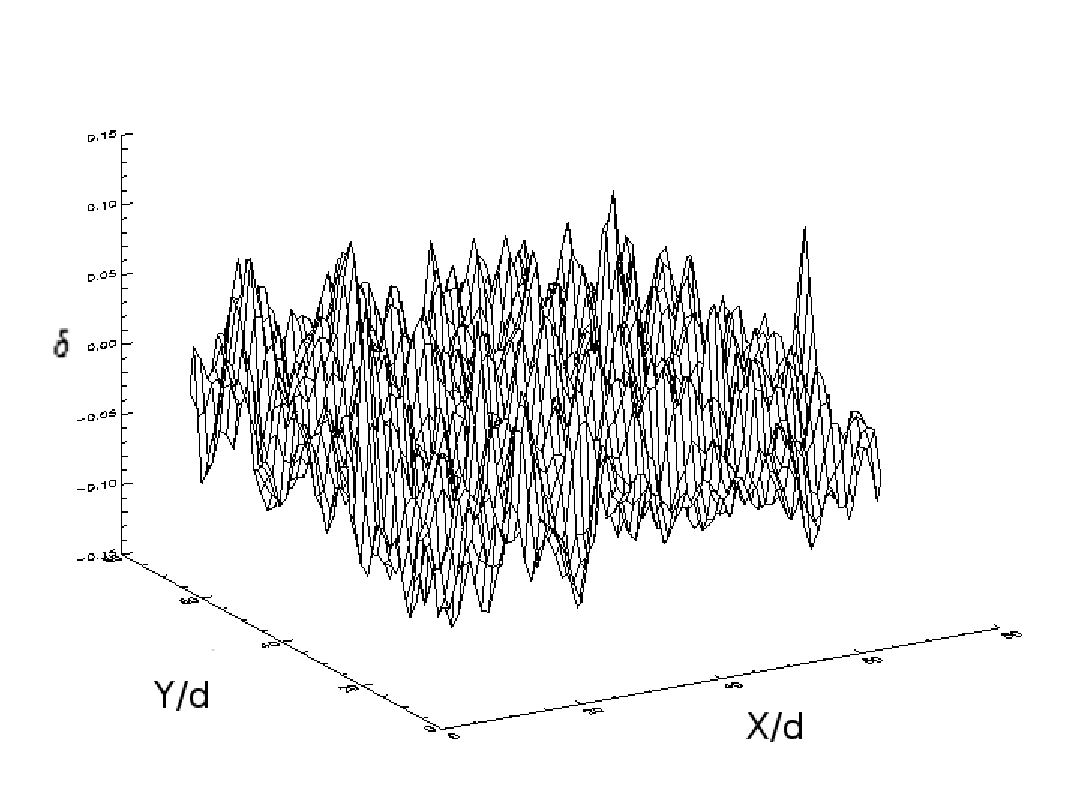
\includegraphics[width=0.49\columnwidth]{./fpa_cos/Delta-0000}
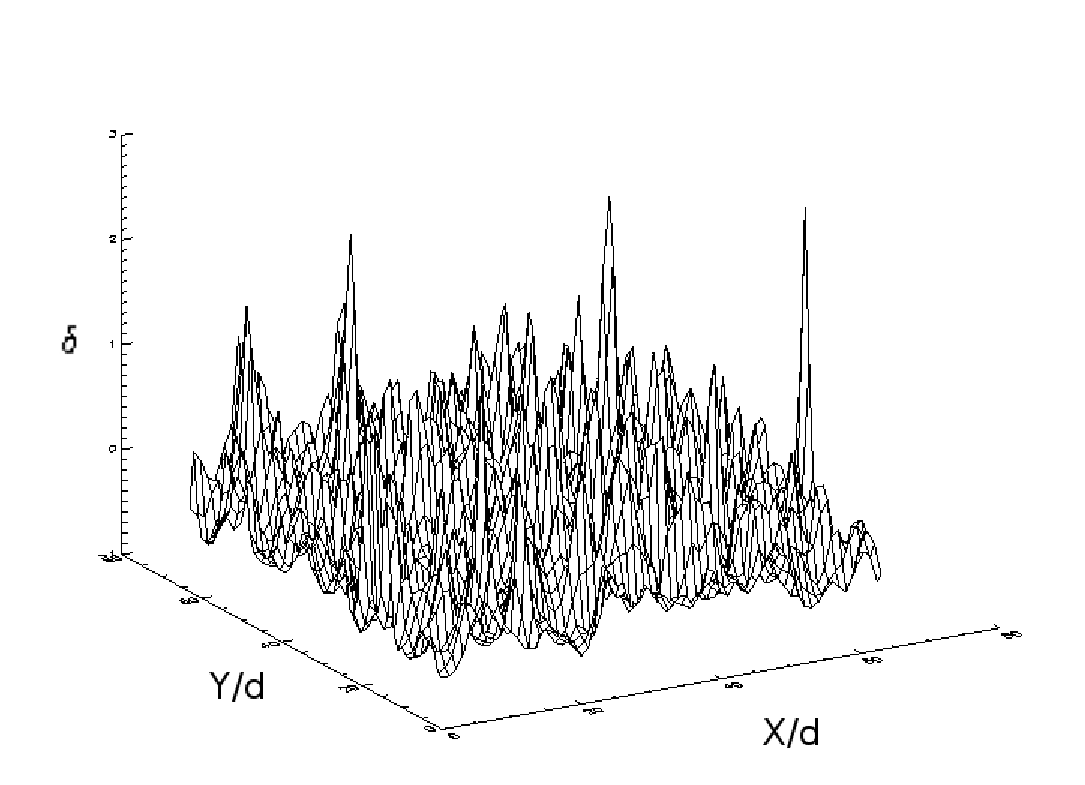
\includegraphics[width=0.49\columnwidth]{./fpa_cos/Delta-0162}
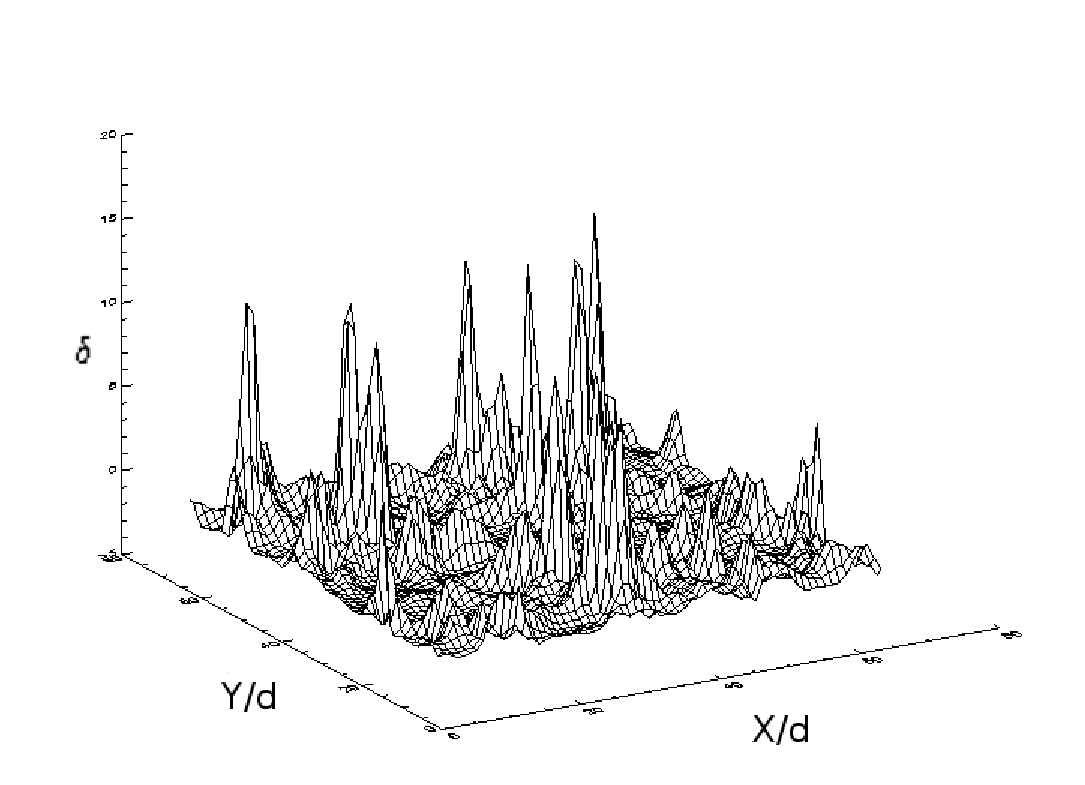
\includegraphics[width=0.49\columnwidth]{./fpa_cos/Delta-0531}
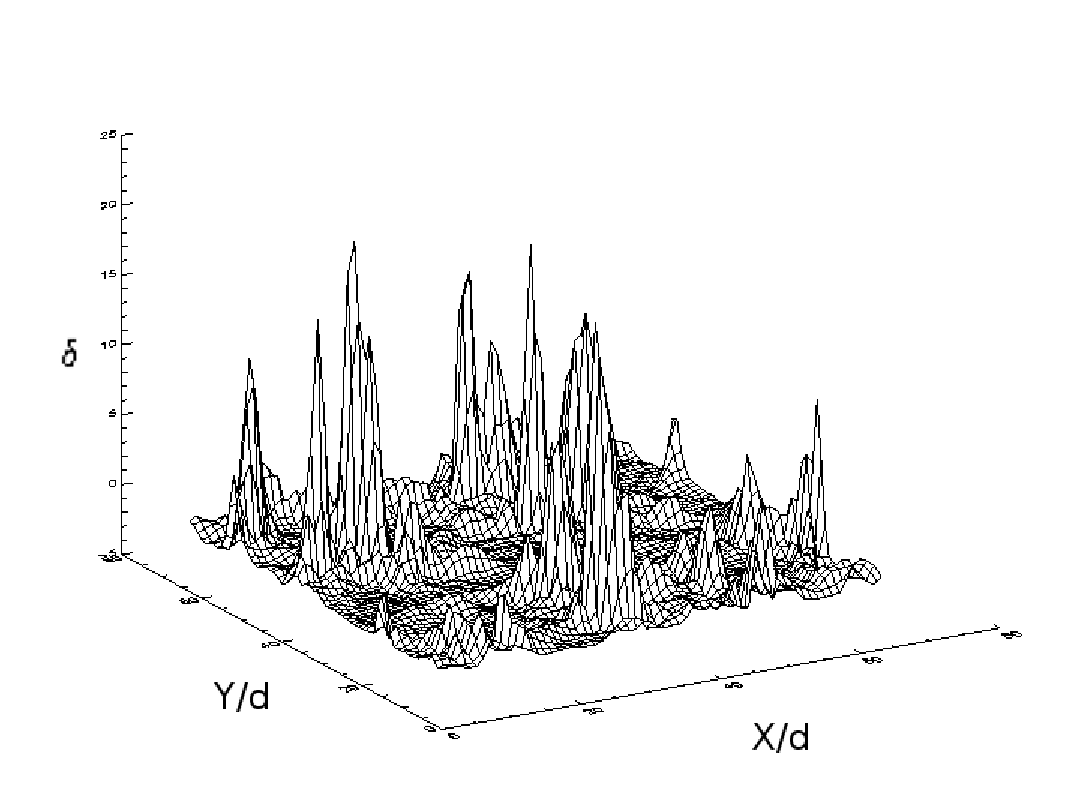
\includegraphics[width=0.49\columnwidth]{./fpa_cos/Delta-0739}
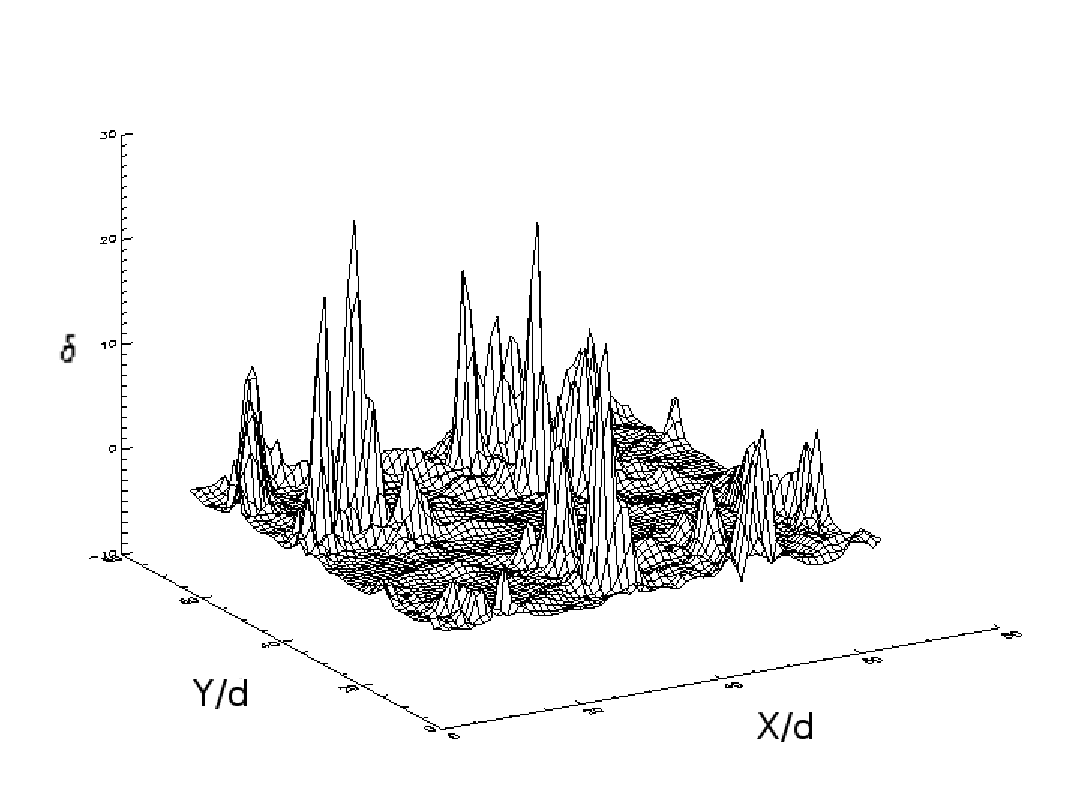
\includegraphics[width=0.49\columnwidth]{./fpa_cos/Delta-0936}

   \end{center}
\caption{The plots here show the evolution of dimensionless density contrast $\delta$ from the 3D FPA code. The $x$ and $y$ axis show dimensionless lengths $x/d$ and $y/d$ as with previous FPA outputs. The output times are $D = 1, 15, 25, 30, 34$. As the simulation evolves we can see structure forming due to gravitational collapse.}
\label{fig.fpa3d}
\end{figure}

\begin{figure}[htb]
   \begin{center}
     %\leavevmode
\includegraphics[width=0.49\columnwidth]{./fpa_cos/hydra/D1001-0162_dc}
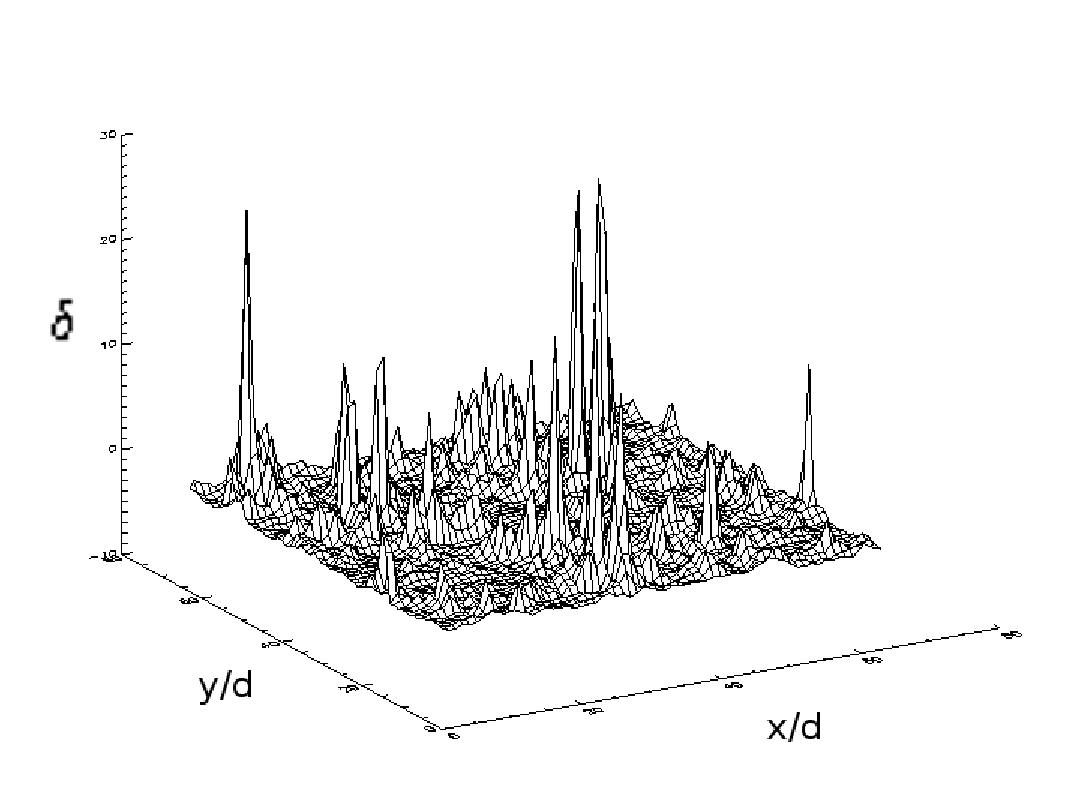
\includegraphics[width=0.49\columnwidth]{./fpa_cos/hydra/D1001-0531_dc}
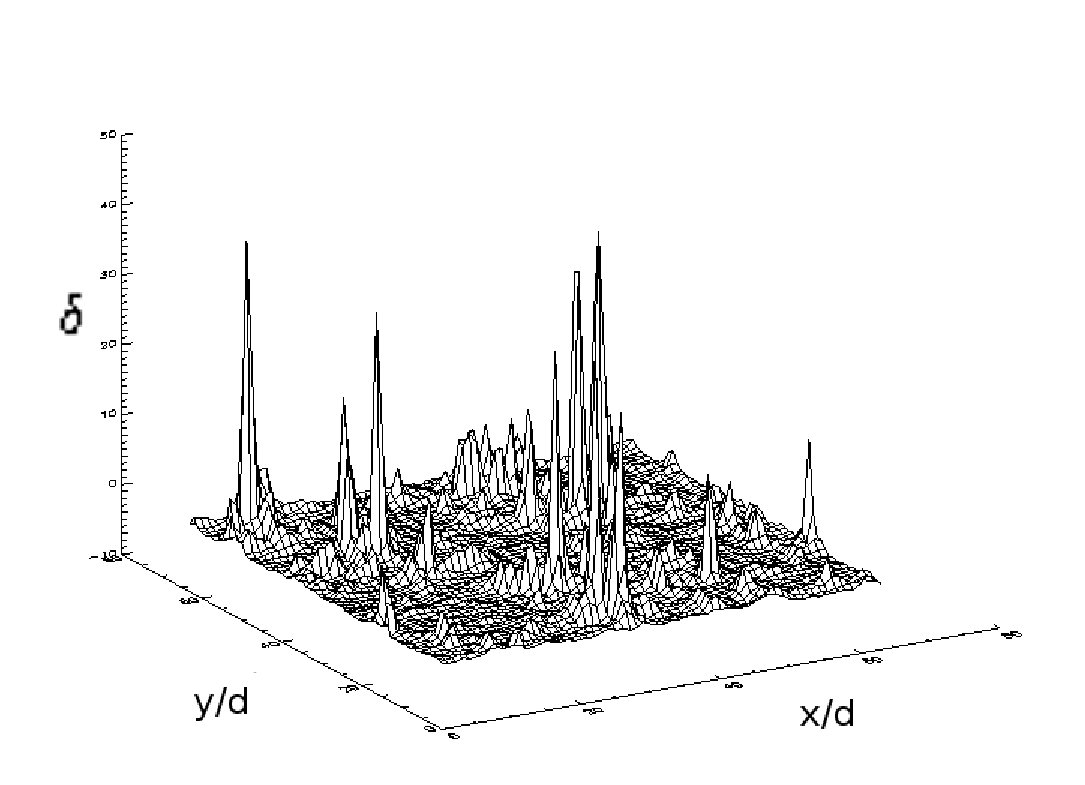
\includegraphics[width=0.49\columnwidth]{./fpa_cos/hydra/D1001-0739_dc}
\includegraphics[width=0.49\columnwidth]{./fpa_cos/hydra/D1001-0936_dc}

   \end{center}
\caption{The plots here show the evolution of density contrast from the Hydra code. The output times correspond to those in the FPA code, they are at timesteps : $t = 162, 531, 739, 936$. Note that the initial density contrast for the two codes is exactly the same hence a plot for timestep 0 ($D=1$) has been omitted from this figure.}
\label{fig.hydra3d}
\end{figure}

\begin{figure}[htb]
   \begin{center}
     %\leavevmode
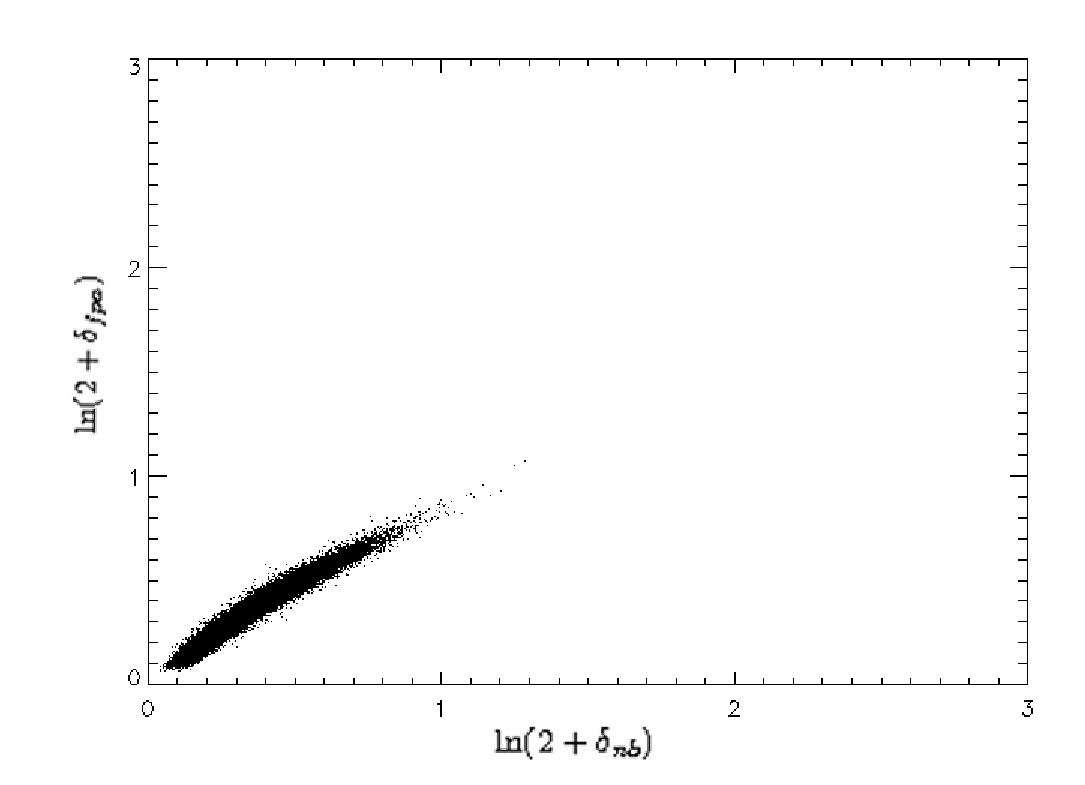
\includegraphics[width=0.49\columnwidth]{./fpa_cos/Lnd_comp_D15_0162_r0-9795}
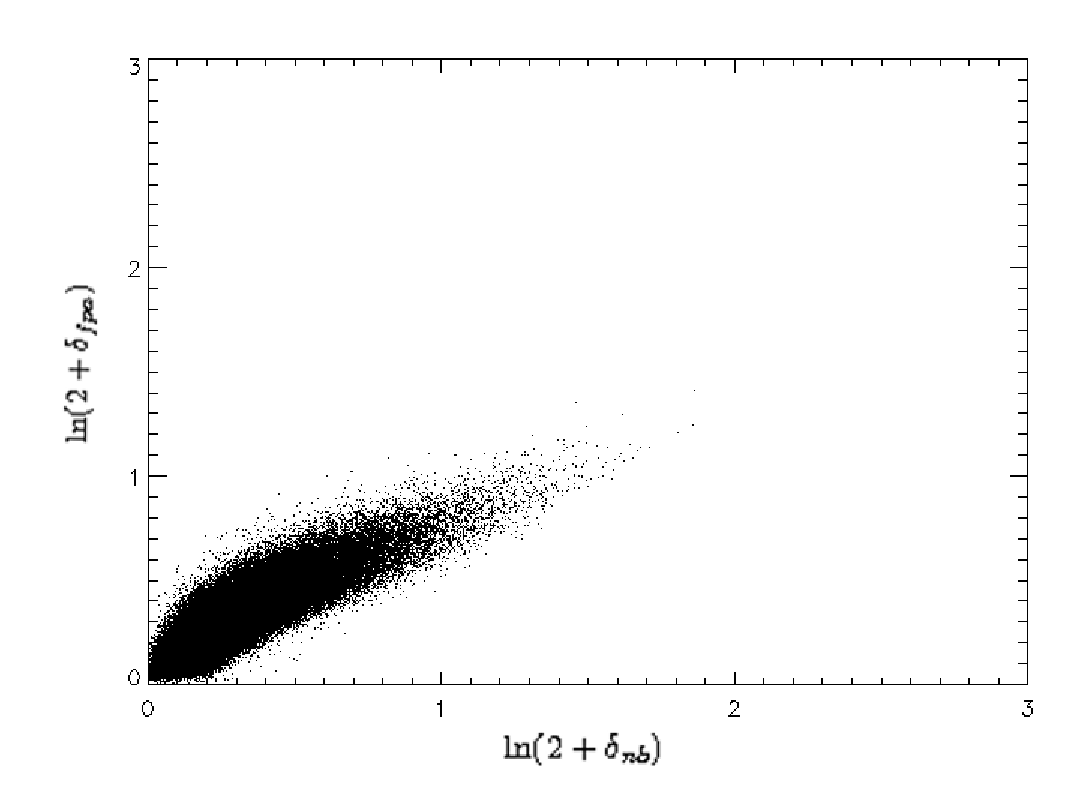
\includegraphics[width=0.49\columnwidth]{./fpa_cos/Lnd_comp_D25_0531_r0-8336}
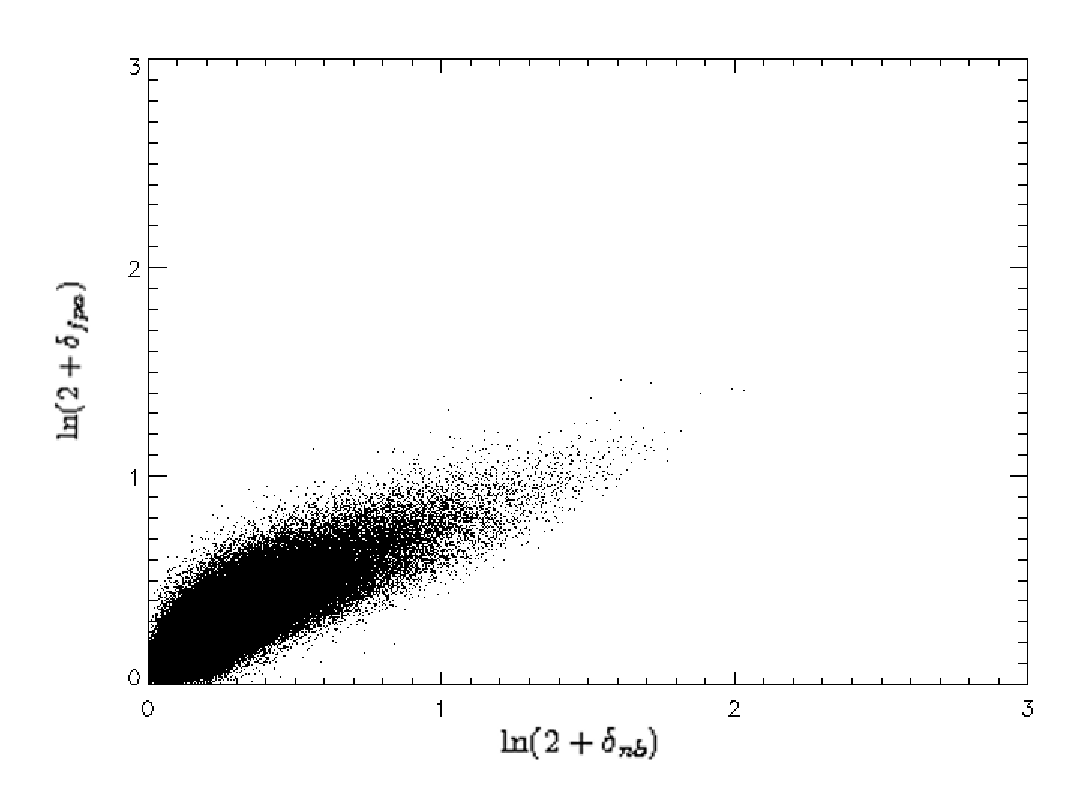
\includegraphics[width=0.49\columnwidth]{./fpa_cos/Lnd_comp_D30_0739_r0-7871}
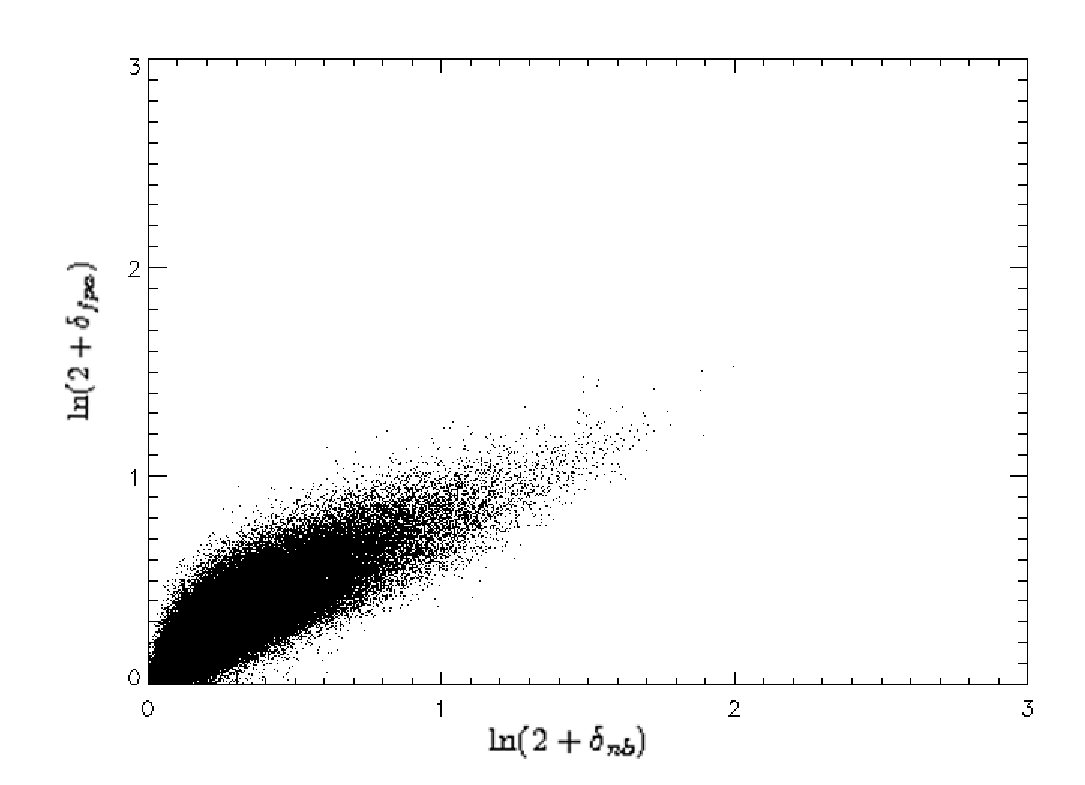
\includegraphics[width=0.49\columnwidth]{./fpa_cos/Lnd_comp_D34_0936_r0-8109}

   \end{center}
\caption{These plots show the correlation between the density contrasts of the $N$-body code (Hydra) and the 3D FPA code. There is a one-to-one correspondence of points from each code, the outputs were matched at the same redshift (that is, time). The x-axis is $\ln(2+ \delta_{nb})$ for Hydra, while the y-axis is  $\ln(2+ \delta_{FPA})$. The correlation coefficients are $r = 0.9795,0.8336, 0.7871, 0.8109$.}
\label{fig.fpacor}
\end{figure}



\subsection{Consistency checks}
As a further test of robustness, we performed a series of checks upon the initial conditions to see if they are consistent with theory. So far we treated the initial conditions generator from Hydra as a black box. We put in cosmological parameters and obtain positions and velocities of the particles (the positions are later turned into density for the FPA code); however, we can examine how well these quantities fit with theory. We expect the histogram of density (and density contrast) to obey a gaussian distribution; although I expect this to be true it is more reliable to check it than just assume it is true. After applying the TSC routine to the positions, we then created a histogram of (over) density and found as gaussian distribution as expected. This is shown in figure \ref{fig.hy_gauss}. Further evidence of this is given by a plot of $\mathcal{I}(\psi) \;{\rm vs}\; \mathcal{R}(\psi)$, as will be shown later in figure \ref{fig.psi_psi}.

We also performed a check of the velocity components which we also expect to be gaussian distributed for each component $x,y,z$. The results of this are shown in the tables below and in figure \ref{fig.hy_vel}. We created histograms for each velocity component and found them to be gaussian, each graph shows an overplot of a theoretical gaussian. The generated velocities are not perfect gaussians but close enough for our purposes. The absolute velocity is shown in the bottom right plot of this figure and it closely follows a Maxwellian distribution as expected. This last plot shows a tighter fit to the underlying theoretical distribution than each of the component velocities. In the tables that follow we tabulate the key parameters of each velocity component.

\vspace*{1cm}
\begin{center}
\begin{tabular}{|r|l|}
  \hline
  quantity & value (km/s) \\ \hline
  max($V_{x}$)  & 169.92818 \\
  min($V_{x}$)  & -184.58659  \\
  mean($V_{x}$) & $9.51\times10^{-9}$ \\
  $\sigma_{v_x}$ & 43.513917 \\
  \hline
\end{tabular}
\end{center}

\begin{center}
\begin{tabular}{|r|l|}
  \hline
  quantity & value (km/s) \\ \hline
  max($V_{y}$)  & 190.18232 \\
  min($V_{y}$)  & -181.42162 \\
  mean($V_{y}$) & $2.888\times10^{-11}$ \\
  $\sigma_{v_y}$ & 43.513917 \\
  \hline
\end{tabular}
\end{center}

\begin{center}
\begin{tabular}{|r|l|}
  \hline
  quantity & value (km/s) \\ \hline
  max($V_{z}$)  & 176.98939 \\
  min($V_{z}$)  & -179.60949 \\
  mean($V_{z}$) & $-2.71\times10^{-9}$ \\
  $\sigma_{v_z}$ & 43.513916 \\
  \hline
\end{tabular}
\end{center}
\vspace*{1cm}

While the maximum and minimum values of velocity are not exactly the same, the velocity dispersions $\sigma_{v_x}, \sigma_{v_y}, \sigma_{v_z}$ are nearly identical across all three axes, agreeing to the 6th decimal place. This near-exact isotropy serves as a strong consistency check on the code. All of the components have mean velocities zero (within machine precision) which denotes that the particles are not experiencing a net bulk motion in some direction. The slight skewing of the distributions is a cause of some concern but the overall behaviour of the simulations are at least believable, hence we do not suspect that something is terribly wrong.

\begin{figure}[htb]
   \begin{center}
     %\leavevmode
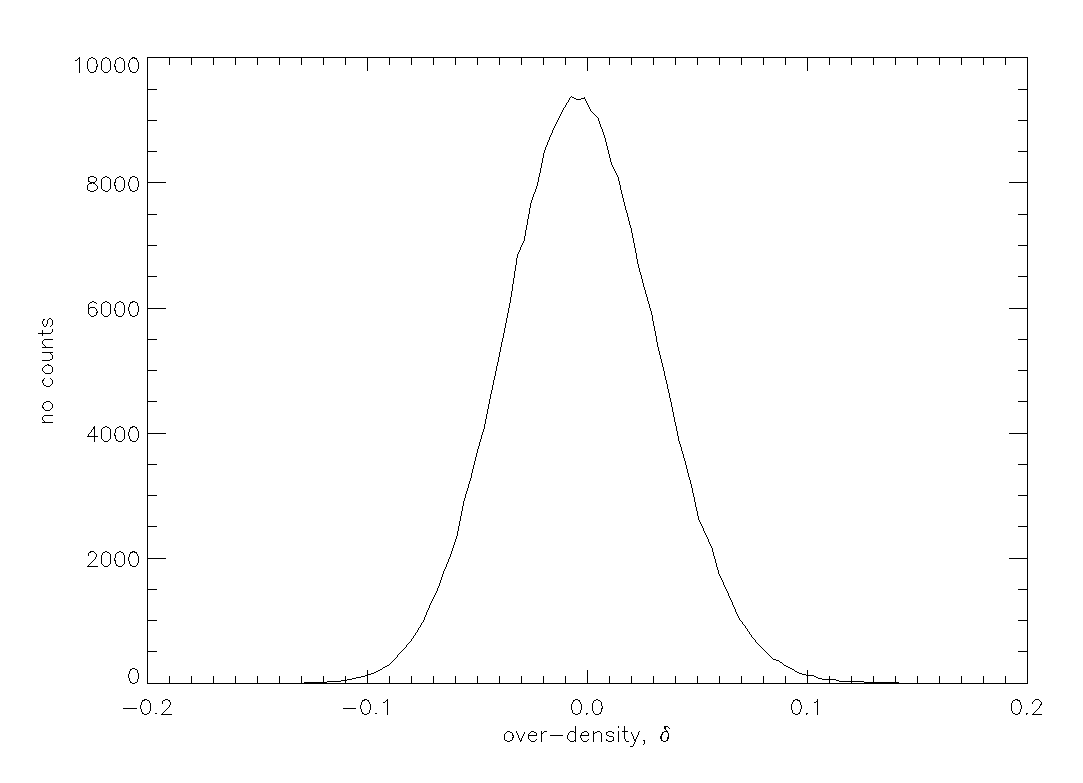
\includegraphics[width=0.49\columnwidth]{./fpa_cos/dc_hist}

   \end{center}
\caption{This plot shows a histogram of density at the start of the simulation. It fits well to a gaussian distribution as expected from theory.}
\label{fig.hy_gauss}
\end{figure}

\begin{figure}[htb]
   \begin{center}
     %\leavevmode
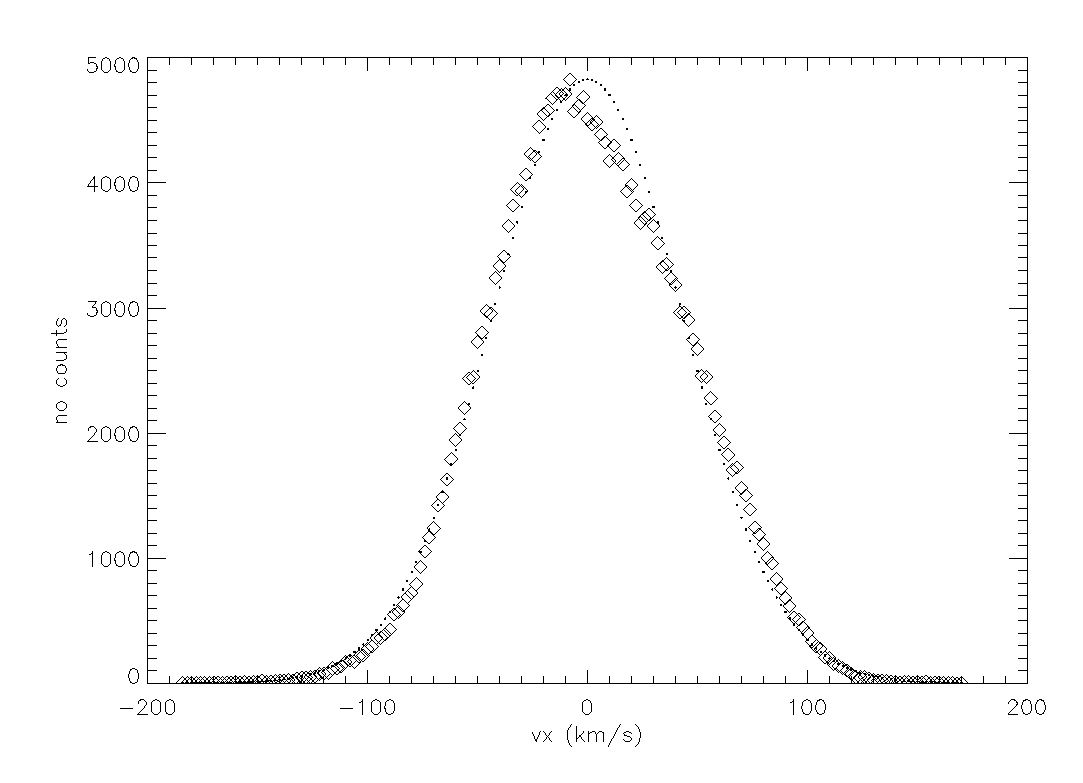
\includegraphics[width=0.49\columnwidth]{./fpa_cos/vel/vx_h_hist}
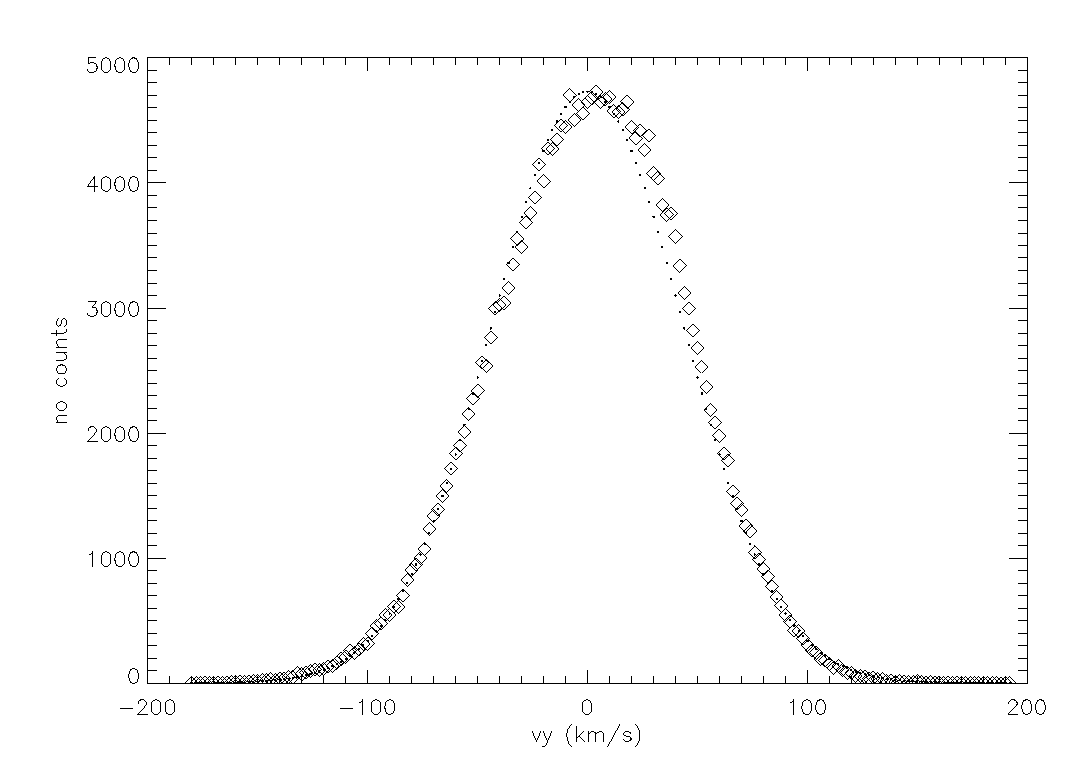
\includegraphics[width=0.49\columnwidth]{./fpa_cos/vel/vy_h_hist}
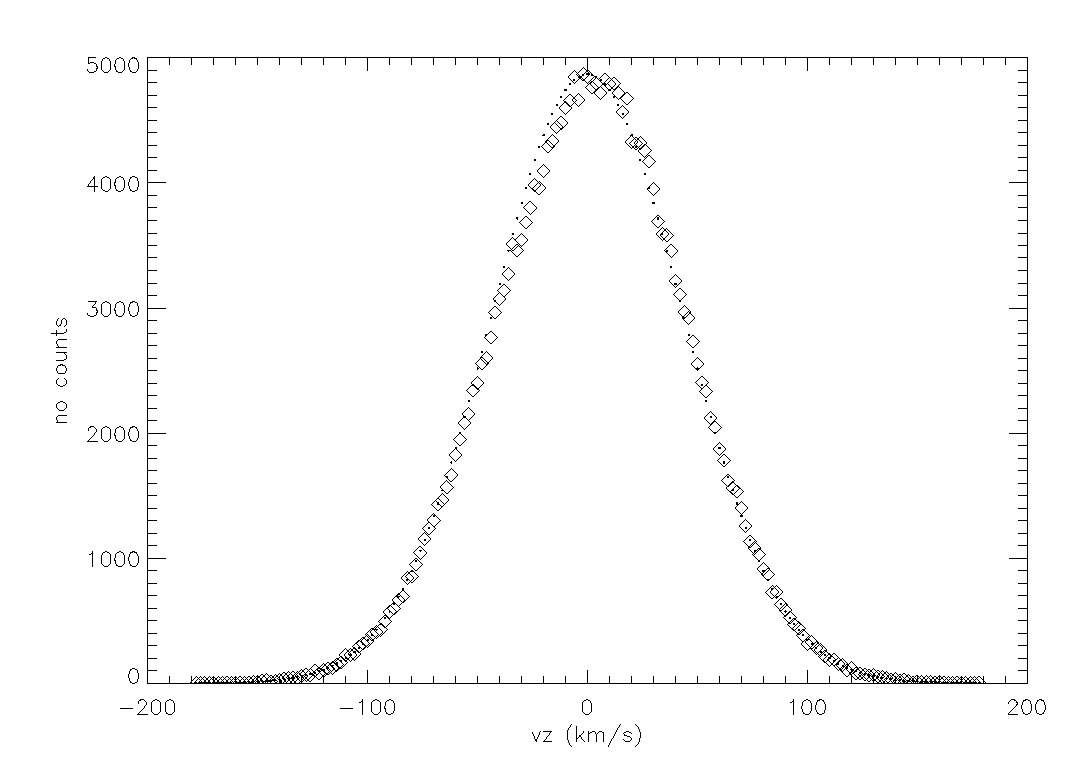
\includegraphics[width=0.49\columnwidth]{./fpa_cos/vel/vz_h_hist}
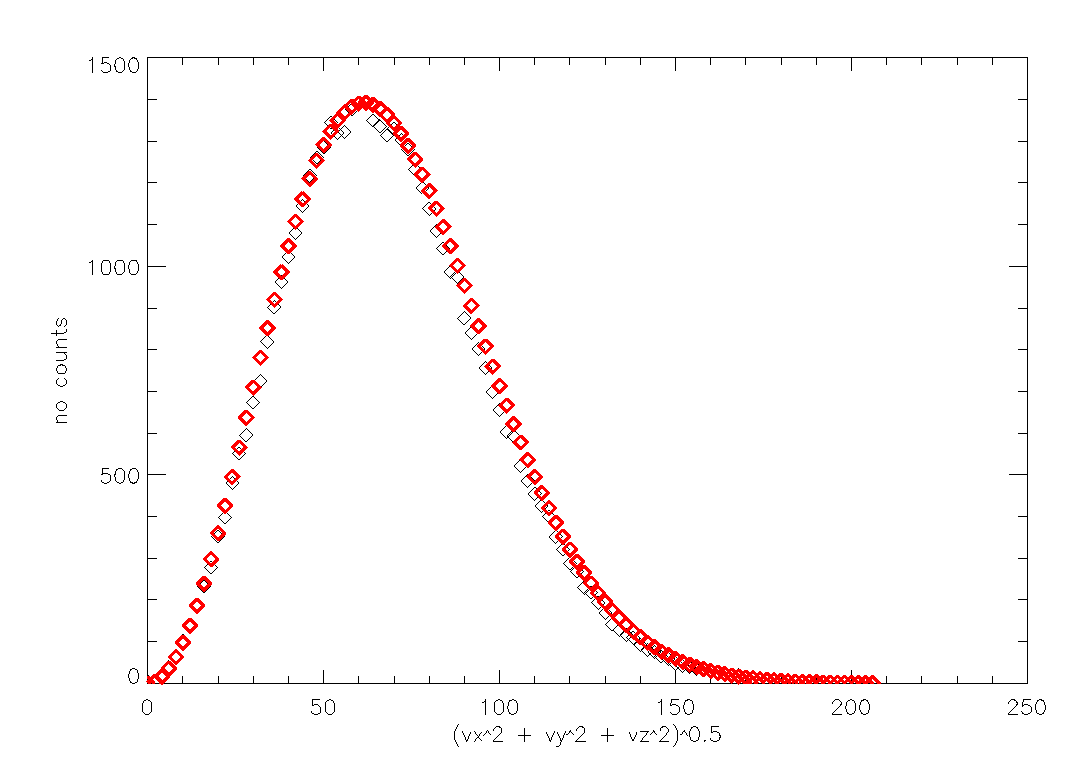
\includegraphics[width=0.49\columnwidth]{./fpa_cos/vel/abs_hist}

   \end{center}
\caption{The plots here show $v_x, v_y, v_z, (v_x^2 + v_y^2 + v_z^2)^{1/2}$ (left-right, top-bottom). The velocity components have a theoretical gaussian overplotted upon them to show how far they deviate from theory. The last plot is overplotted with a theoretical Maxwellian curve which shows a tight comparison between the generated velocity distribution and the expected distribution from theory.}
\label{fig.hy_vel}
\end{figure}

An interesting artefact of wave-mechanics is the apparent deformation of velocities when constructing the wavefunction. From the FPA code, we constructed the velocity field from the probability current (equation \ref{eqn_j}) and then plotted the output against that from the $N$-body code. Figure \ref{fig.hy_fpa_vel} shows a simple point-by-point comparison of the $v_x$ components from the two codes.

\begin{figure}[htb]
   \begin{center}
     %\leavevmode
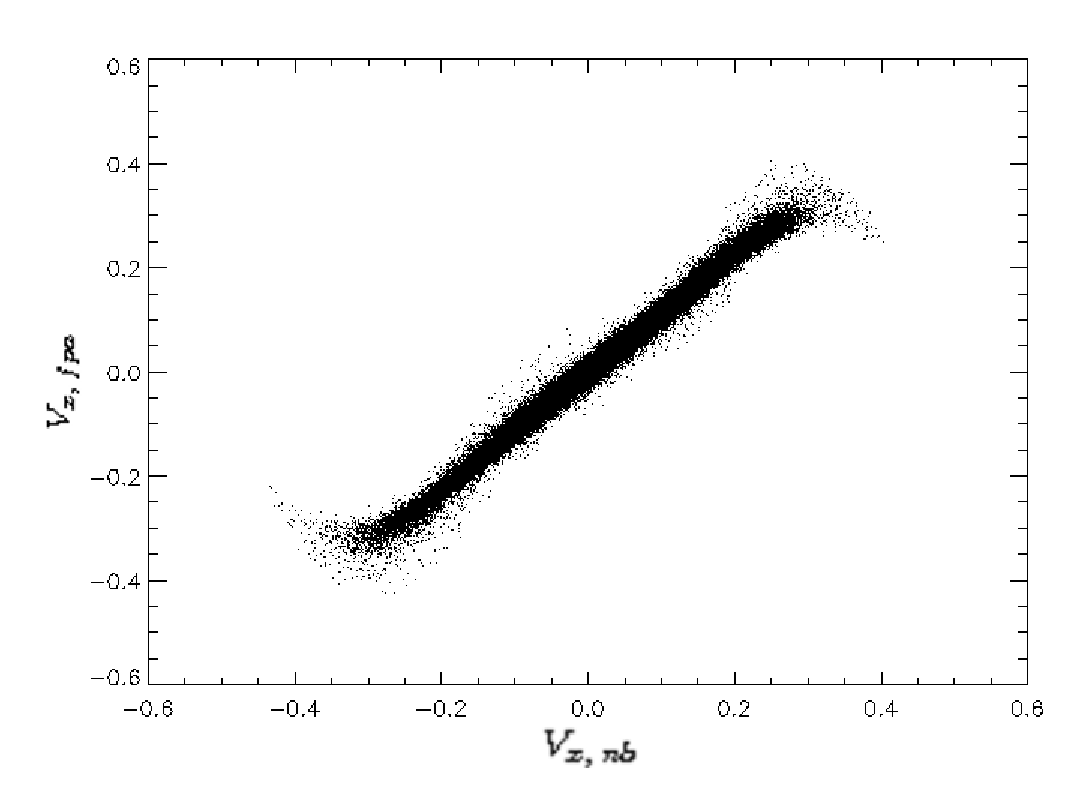
\includegraphics[width=0.49\columnwidth]{./fpa_cos/vel/Vx_comp_1}

   \end{center}
\caption{Point-by-point comparison of $v_x$ components: $N$-body (x-axis) vs FPA (y-axis) in the initial conditions. The central region shows the expected tight linear correlation. The turn-over at the extremes of the velocity range is an artefact of constructing the wavefunction: the phase wrapping at large velocities (where $|v| \to \pi\nu/\Delta x$) aliases the velocity, causing a roll-off rather than the expected linear continuation.}

\label{fig.hy_fpa_vel}
\end{figure}


\subsection{Vorticity}
\label{ch4vort}
In section \ref{vort} we mentioned the possibility of detecting vorticity in our velocity outputs. From theory we do not expect vorticity to exist, hence the presence of vortices in our results may indicate when the code has reached the end of its reliability. As previously mentioned, we expect to find the centre of a vortex at a gridpoint where the velocity is undefined. That is when $v = \nabla\phi$ no longer makes sense. This occurs most obviously when $\psi = (0,0), \;\psi\in\mathbb{C}$ which corresponds to a region of no density: that is a vortical void. Such a region is easy to find computationally. For illustrative purposes I will present graphs of $\mathcal{I}(\psi) \;{\rm vs}\; \mathcal{R}(\psi)$ at 3 different linear growth factors $D = 1, 10, 30$.

At the initial time the distribution of points of the wavefunction corroborate with the fact that the density and velocity follow a gaussian distribution. The circular ring we see has unit radius and the points appear to be even in distribution. At later times the distribution is still evenly distributed (a statement that physics is acting isotropically as required) but the points are no longer a tight ring but smeared out. Eventually the distribution has a closer resemblance to a solid circle. Only at the later times we will see a gridpoint where $\psi = (0,0)$ and hence possibly detect vorticity. From figure \ref{fig.psi_psi} we can see that at $D = 30$ there is potentially a number of gridpoints that are very close to zero.

In figure \ref{fig.vort} we can see an $x-y$ slice at some $z$ of the velocity field. This slice contains a point where the wavefunction is zero — a potential candidate for vorticity. If we look carefully we can see an anomalous velocity vector that has far greater magnitude than the rest of the field. If we zoom into to look closer at this slice then we can see the rest of the velocity vectors `circling' around the wavefunctions null-point.

\begin{figure}[htb]
   \begin{center}
     %\leavevmode
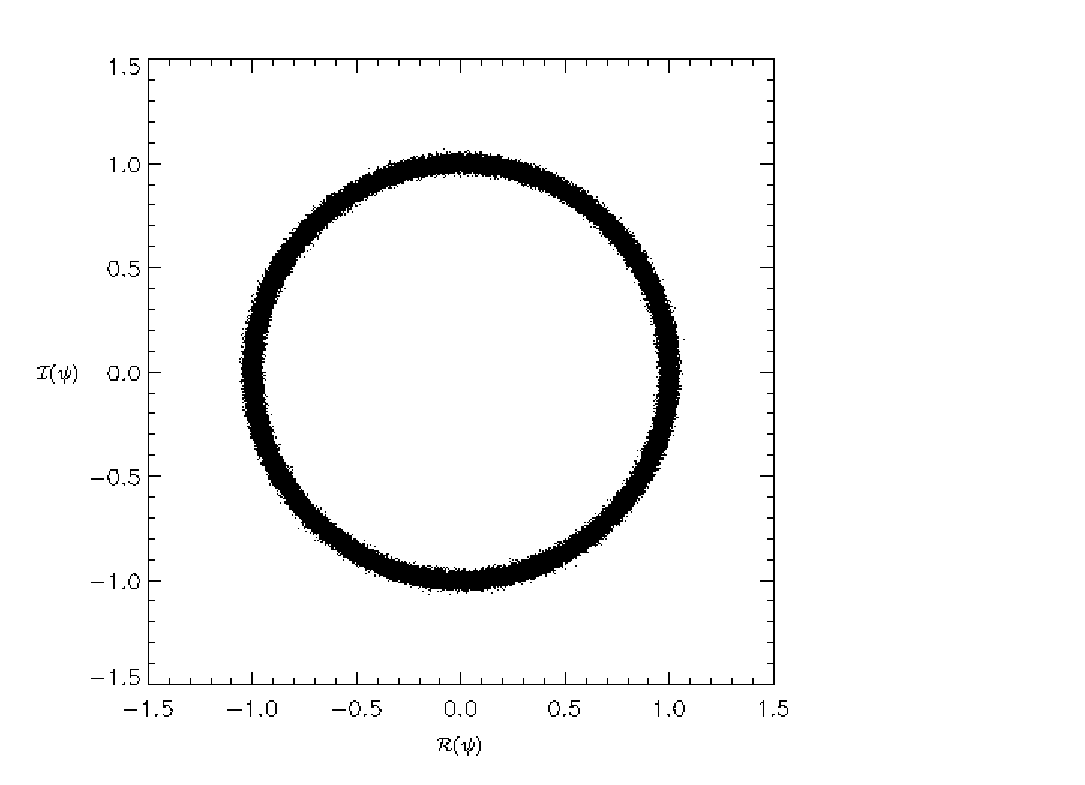
\includegraphics[width=0.49\columnwidth]{./fpa_cos/psi_D1}
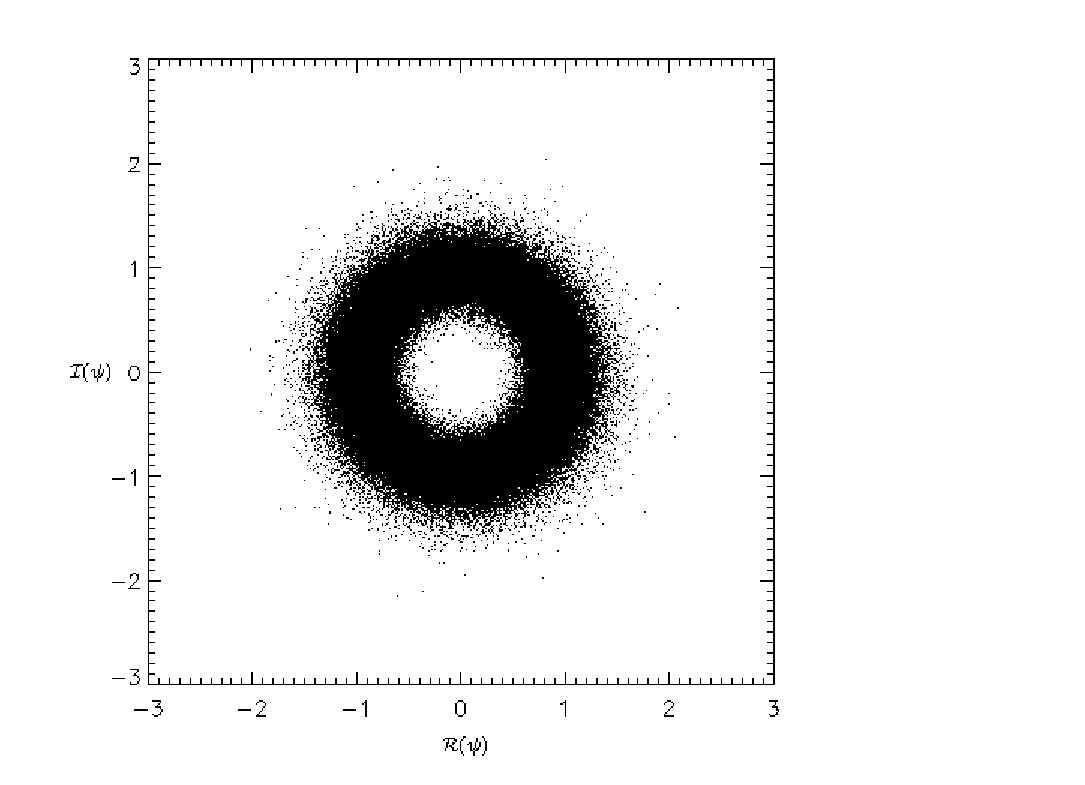
\includegraphics[width=0.49\columnwidth]{./fpa_cos/psi_D10}
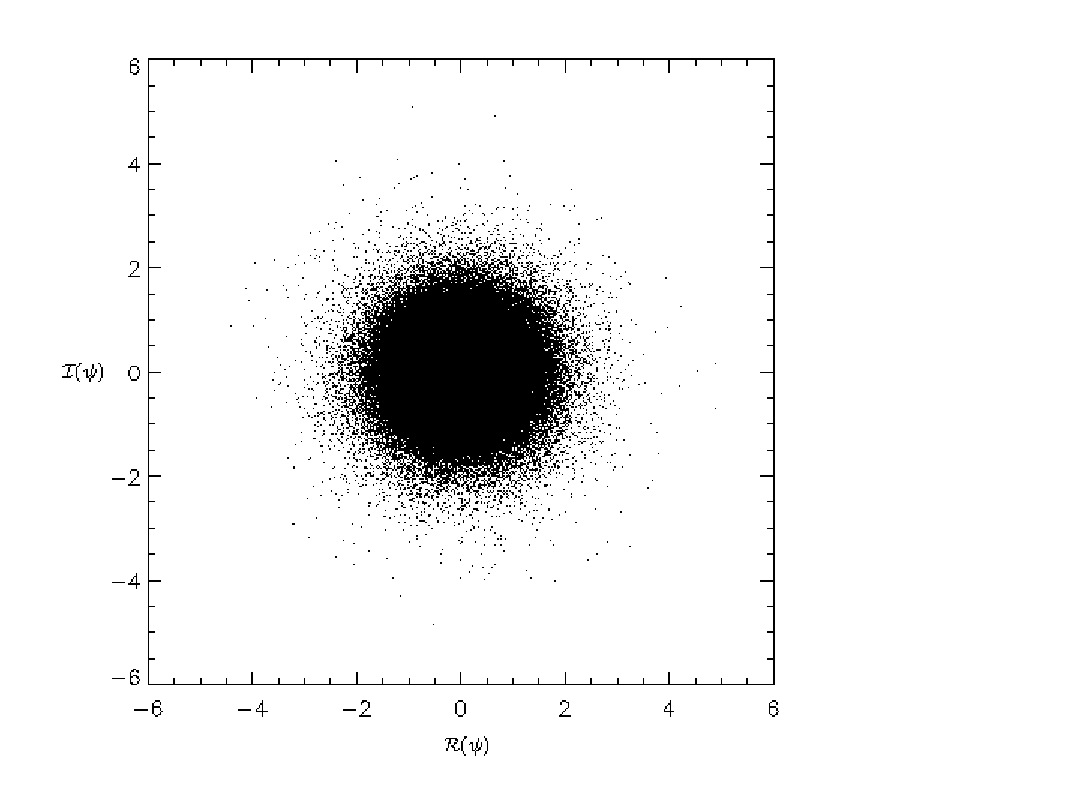
\includegraphics[width=0.49\columnwidth]{./fpa_cos/psi_D30}

   \end{center}
\caption{The plots show $\mathcal{I}(\psi) \;{\rm vs}\; \mathcal{R}(\psi)$ at growth factors $D = 1, 10, 30$. The first plot shows a ring of unit radius as expected from the initial conditions generator. The smearing out of this ring is indicative that the wavefunction is evolving and hence the over-densities are spread further from the mean.}
\label{fig.psi_psi}
\end{figure}


\begin{figure}[htb]
   \begin{center}
     %\leavevmode
\includegraphics[width=0.49\columnwidth]{./fpa_cos/vel/Vel_field}
\includegraphics[width=0.49\columnwidth]{./fpa_cos/vel/Vel_field_zoom}

   \end{center}
\caption{The left plot shows a slice of $x$ and $y$ components of the velocity at time $D = 30$ (showing array element on each axes). On the right is a plot that zooms in, and centres, upon the gridpoint where the velocity vector is largest.}
\label{fig.vort}
\end{figure}


%
%  Conclusion of FPA
%
\section{Conclusion and evaluation of FPA}
The FPA is a fast and efficient method for probing the quasi-linear regime of density perturbations, and proves to be a good match for the Zel'dovich approximation, though like the Zel'dovich method it breaks down at shell crossing. The 1D and 3D toy models were a demonstration of the mathematics providing a consistent framework that is able to be coded in such way that gravity (from the Poisson equation) can be coupled to the Schr\"odinger equation.

After testing the toy models, I have confirmed that the FPA can handle `real' cosmological initial conditions and provide simulation results that are comparable to the widely available $N$-body codes (at least in the quasi-linear regime). The benefit of the FPA is that, in the quasi-linear regime, it runs much faster than $N$-body codes as it can jump directly to any growth factor without computing intermediate time steps.

\subsection{From FPA to solving the full system}
To plan our subsequent work it is useful to consider the weaker points of the FPA, such as the inability of the FPA to probe far beyond the linear regime. Like the Zel'dovich approximation it breaks down at high densities. In the dense regions where shell crossing occurs, singularities in density prevent the code from being reliable after shell crossing. The evolution, essentially, becomes `stuck' and does not progress after such a time. This can be circumvented by solving the full Schr\"odinger-Poisson system which allows for multi-streaming (density peaks can pass through one another).

As an extension to the FPA, Short tried a perturbative approach as presented in Chapter 5 of his thesis. This involved adding a perturbation term to the free particle Hamiltonian. The effective potential is still set to zero, so this approach will only allow for small deviations from the kinetic energy term of the free particle Hamiltonian. This approach is still valid in the FPA framework, hence the code can still jump to any time step. Including the potential term in the Hamiltonian is a non-perturbative approach and is consequently much slower as each intermediate time step has to be calculated. In the next Chapter I present my solution to tackling the full Schr\"odinger-Poisson system.



